%% bare_jrnl.tex
%% V1.4a
%% 2014/09/17
%% by Michael Shell
%% see http://www.michaelshell.org/
%% for current contact information.
%%
%% This is a skeleton file demonstrating the use of IEEEtran.cls
%% (requires IEEEtran.cls version 1.8a or later) with an IEEE
%% journal paper.
%%
%% Support sites:
%% http://www.michaelshell.org/tex/ieeetran/
%% http://www.ctan.org/tex-archive/macros/latex/contrib/IEEEtran/
%% and
%% http://www.ieee.org/

%%*************************************************************************
%% Legal Notice:
%% This code is offered as-is without any warranty either expressed or
%% implied; without even the implied warranty of MERCHANTABILITY or
%% FITNESS FOR A PARTICULAR PURPOSE! 
%% User assumes all risk.
%% In no event shall IEEE or any contributor to this code be liable for
%% any damages or losses, including, but not limited to, incidental,
%% consequential, or any other damages, resulting from the use or misuse
%% of any information contained here.
%%
%% All comments are the opinions of their respective authors and are not
%% necessarily endorsed by the IEEE.
%%
%% This work is distributed under the LaTeX Project Public License (LPPL)
%% ( http://www.latex-project.org/ ) version 1.3, and may be freely used,
%% distributed and modified. A copy of the LPPL, version 1.3, is included
%% in the base LaTeX documentation of all distributions of LaTeX released
%% 2003/12/01 or later.
%% Retain all contribution notices and credits.
%% ** Modified files should be clearly indicated as such, including  **
%% ** renaming them and changing author support contact information. **
%%
%% File list of work: IEEEtran.cls, IEEEtran_HOWTO.pdf, bare_adv.tex,
%%                    bare_conf.tex, bare_jrnl.tex, bare_conf_compsoc.tex,
%%                    bare_jrnl_compsoc.tex, bare_jrnl_transmag.tex
%%*************************************************************************


% *** Authors should verify (and, if needed, correct) their LaTeX system  ***
% *** with the testflow diagnostic prior to trusting their LaTeX platform ***
% *** with production work. IEEE's font choices and paper sizes can       ***
% *** trigger bugs that do not appear when using other class files.       ***                          ***
% The testflow support page is at:
% http://www.michaelshell.org/tex/testflow/



\documentclass[journal]{IEEEtran}
%
% If IEEEtran.cls has not been installed into the LaTeX system files,
% manually specify the path to it like:
% \documentclass[journal]{../sty/IEEEtran}





% Some very useful LaTeX packages include:
% (uncomment the ones you want to load)


% *** MISC UTILITY PACKAGES ***
%
%\usepackage{ifpdf}
% Heiko Oberdiek's ifpdf.sty is very useful if you need conditional
% compilation based on whether the output is pdf or dvi.
% usage:
% \ifpdf
%   % pdf code
% \else
%   % dvi code
% \fi
% The latest version of ifpdf.sty can be obtained from:
% http://www.ctan.org/tex-archive/macros/latex/contrib/oberdiek/
% Also, note that IEEEtran.cls V1.7 and later provides a builtin
% \ifCLASSINFOpdf conditional that works the same way.
% When switching from latex to pdflatex and vice-versa, the compiler may
% have to be run twice to clear warning/error messages.


\usepackage{tabu}
%\usepackage{caption}
\usepackage[font={small,it}]{caption}
\usepackage[affil-it]{authblk}
\usepackage[utf8]{inputenc}
\usepackage{array}
\usepackage{makecell}
\usepackage{url}

% *** CITATION PACKAGES ***
%
%\usepackage{cite}
% cite.sty was written by Donald Arseneau
% V1.6 and later of IEEEtran pre-defines the format of the cite.sty package
% \cite{} output to follow that of IEEE. Loading the cite package will
% result in citation numbers being automatically sorted and properly
% "compressed/ranged". e.g., [1], [9], [2], [7], [5], [6] without using
% cite.sty will become [1], [2], [5]--[7], [9] using cite.sty. cite.sty's
% \cite will automatically add leading space, if needed. Use cite.sty's
% noadjust option (cite.sty V3.8 and later) if you want to turn this off
% such as if a citation ever needs to be enclosed in parenthesis.
% cite.sty is already installed on most LaTeX systems. Be sure and use
% version 5.0 (2009-03-20) and later if using hyperref.sty.
% The latest version can be obtained at:
% http://www.ctan.org/tex-archive/macros/latex/contrib/cite/
% The documentation is contained in the cite.sty file itself.






% *** GRAPHICS RELATED PACKAGES ***
%
\ifCLASSINFOpdf
 \usepackage[pdftex]{graphicx}
  % declare the path(s) where your graphic files are
  \graphicspath{{C:/Users/Alex/Documents/R/ravelry/analysis/}}
  % and their extensions so you won't have to specify these with
  % every instance of \includegraphics
  % \DeclareGraphicsExtensions{.pdf,.jpeg,.png}
\else
  % or other class option (dvipsone, dvipdf, if not using dvips). graphicx
  % will default to the driver specified in the system graphics.cfg if no
  % driver is specified.
  % \usepackage[dvips]{graphicx}
  % declare the path(s) where your graphic files are
  % \graphicspath{{../eps/}}
  % and their extensions so you won't have to specify these with
  % every instance of \includegraphics
  % \DeclareGraphicsExtensions{.eps}
\fi
% graphicx was written by David Carlisle and Sebastian Rahtz. It is
% required if you want graphics, photos, etc. graphicx.sty is already
% installed on most LaTeX systems. The latest version and documentation
% can be obtained at: 
% http://www.ctan.org/tex-archive/macros/latex/required/graphics/
% Another good source of documentation is "Using Imported Graphics in
% LaTeX2e" by Keith Reckdahl which can be found at:
% http://www.ctan.org/tex-archive/info/epslatex/
%
% latex, and pdflatex in dvi mode, support graphics in encapsulated
% postscript (.eps) format. pdflatex in pdf mode supports graphics
% in .pdf, .jpeg, .png and .mps (metapost) formats. Users should ensure
% that all non-photo figures use a vector format (.eps, .pdf, .mps) and
% not a bitmapped formats (.jpeg, .png). IEEE frowns on bitmapped formats
% which can result in "jaggedy"/blurry rendering of lines and letters as
% well as large increases in file sizes.
%
% You can find documentation about the pdfTeX application at:
% http://www.tug.org/applications/pdftex





% *** MATH PACKAGES ***
%
%\usepackage[cmex10]{amsmath}
% A popular package from the American Mathematical Society that provides
% many useful and powerful commands for dealing with mathematics. If using
% it, be sure to load this package with the cmex10 option to ensure that
% only type 1 fonts will utilized at all point sizes. Without this option,
% it is possible that some math symbols, particularly those within
% footnotes, will be rendered in bitmap form which will result in a
% document that can not be IEEE Xplore compliant!
%
% Also, note that the amsmath package sets \interdisplaylinepenalty to 10000
% thus preventing page breaks from occurring within multiline equations. Use:
%\interdisplaylinepenalty=2500
% after loading amsmath to restore such page breaks as IEEEtran.cls normally
% does. amsmath.sty is already installed on most LaTeX systems. The latest
% version and documentation can be obtained at:
% http://www.ctan.org/tex-archive/macros/latex/required/amslatex/math/





% *** SPECIALIZED LIST PACKAGES ***
%
%\usepackage{algorithmic}
% algorithmic.sty was written by Peter Williams and Rogerio Brito.
% This package provides an algorithmic environment fo describing algorithms.
% You can use the algorithmic environment in-text or within a figure
% environment to provide for a floating algorithm. Do NOT use the algorithm
% floating environment provided by algorithm.sty (by the same authors) or
% algorithm2e.sty (by Christophe Fiorio) as IEEE does not use dedicated
% algorithm float types and packages that provide these will not provide
% correct IEEE style captions. The latest version and documentation of
% algorithmic.sty can be obtained at:
% http://www.ctan.org/tex-archive/macros/latex/contrib/algorithms/
% There is also a support site at:
% http://algorithms.berlios.de/index.html
% Also of interest may be the (relatively newer and more customizable)
% algorithmicx.sty package by Szasz Janos:
% http://www.ctan.org/tex-archive/macros/latex/contrib/algorithmicx/




% *** ALIGNMENT PACKAGES ***
%
%\usepackage{array}
% Frank Mittelbach's and David Carlisle's array.sty patches and improves
% the standard LaTeX2e array and tabular environments to provide better
% appearance and additional user controls. As the default LaTeX2e table
% generation code is lacking to the point of almost being broken with
% respect to the quality of the end results, all users are strongly
% advised to use an enhanced (at the very least that provided by array.sty)
% set of table tools. array.sty is already installed on most systems. The
% latest version and documentation can be obtained at:
% http://www.ctan.org/tex-archive/macros/latex/required/tools/


% IEEEtran contains the IEEEeqnarray family of commands that can be used to
% generate multiline equations as well as matrices, tables, etc., of high
% quality.




% *** SUBFIGURE PACKAGES ***
%\ifCLASSOPTIONcompsoc
%  \usepackage[caption=false,font=normalsize,labelfont=sf,textfont=sf]{subfig}
%\else
%  \usepackage[caption=false,font=footnotesize]{subfig}
%\fi
% subfig.sty, written by Steven Douglas Cochran, is the modern replacement
% for subfigure.sty, the latter of which is no longer maintained and is
% incompatible with some LaTeX packages including fixltx2e. However,
% subfig.sty requires and automatically loads Axel Sommerfeldt's caption.sty
% which will override IEEEtran.cls' handling of captions and this will result
% in non-IEEE style figure/table captions. To prevent this problem, be sure
% and invoke subfig.sty's "caption=false" package option (available since
% subfig.sty version 1.3, 2005/06/28) as this is will preserve IEEEtran.cls
% handling of captions.
% Note that the Computer Society format requires a larger sans serif font
% than the serif footnote size font used in traditional IEEE formatting
% and thus the need to invoke different subfig.sty package options depending
% on whether compsoc mode has been enabled.
%
% The latest version and documentation of subfig.sty can be obtained at:
% http://www.ctan.org/tex-archive/macros/latex/contrib/subfig/




% *** FLOAT PACKAGES ***
%
%\usepackage{fixltx2e}
% fixltx2e, the successor to the earlier fix2col.sty, was written by
% Frank Mittelbach and David Carlisle. This package corrects a few problems
% in the LaTeX2e kernel, the most notable of which is that in current
% LaTeX2e releases, the ordering of single and double column floats is not
% guaranteed to be preserved. Thus, an unpatched LaTeX2e can allow a
% single column figure to be placed prior to an earlier double column
% figure. The latest version and documentation can be found at:
% http://www.ctan.org/tex-archive/macros/latex/base/


%\usepackage{stfloats}
% stfloats.sty was written by Sigitas Tolusis. This package gives LaTeX2e
% the ability to do double column floats at the bottom of the page as well
% as the top. (e.g., "\begin{figure*}[!b]" is not normally possible in
% LaTeX2e). It also provides a command:
%\fnbelowfloat
% to enable the placement of footnotes below bottom floats (the standard
% LaTeX2e kernel puts them above bottom floats). This is an invasive package
% which rewrites many portions of the LaTeX2e float routines. It may not work
% with other packages that modify the LaTeX2e float routines. The latest
% version and documentation can be obtained at:
% http://www.ctan.org/tex-archive/macros/latex/contrib/sttools/
% Do not use the stfloats baselinefloat ability as IEEE does not allow
% \baselineskip to stretch. Authors submitting work to the IEEE should note
% that IEEE rarely uses double column equations and that authors should try
% to avoid such use. Do not be tempted to use the cuted.sty or midfloat.sty
% packages (also by Sigitas Tolusis) as IEEE does not format its papers in
% such ways.
% Do not attempt to use stfloats with fixltx2e as they are incompatible.
% Instead, use Morten Hogholm'a dblfloatfix which combines the features
% of both fixltx2e and stfloats:
%
% \usepackage{dblfloatfix}
% The latest version can be found at:
% http://www.ctan.org/tex-archive/macros/latex/contrib/dblfloatfix/




%\ifCLASSOPTIONcaptionsoff
%  \usepackage[nomarkers]{endfloat}
% \let\MYoriglatexcaption\caption
% \renewcommand{\caption}[2][\relax]{\MYoriglatexcaption[#2]{#2}}
%\fi
% endfloat.sty was written by James Darrell McCauley, Jeff Goldberg and 
% Axel Sommerfeldt. This package may be useful when used in conjunction with 
% IEEEtran.cls'  captionsoff option. Some IEEE journals/societies require that
% submissions have lists of figures/tables at the end of the paper and that
% figures/tables without any captions are placed on a page by themselves at
% the end of the document. If needed, the draftcls IEEEtran class option or
% \CLASSINPUTbaselinestretch interface can be used to increase the line
% spacing as well. Be sure and use the nomarkers option of endfloat to
% prevent endfloat from "marking" where the figures would have been placed
% in the text. The two hack lines of code above are a slight modification of
% that suggested by in the endfloat docs (section 8.4.1) to ensure that
% the full captions always appear in the list of figures/tables - even if
% the user used the short optional argument of \caption[]{}.
% IEEE papers do not typically make use of \caption[]'s optional argument,
% so this should not be an issue. A similar trick can be used to disable
% captions of packages such as subfig.sty that lack options to turn off
% the subcaptions:
% For subfig.sty:
% \let\MYorigsubfloat\subfloat
% \renewcommand{\subfloat}[2][\relax]{\MYorigsubfloat[]{#2}}
% However, the above trick will not work if both optional arguments of
% the \subfloat command are used. Furthermore, there needs to be a
% description of each subfigure *somewhere* and endfloat does not add
% subfigure captions to its list of figures. Thus, the best approach is to
% avoid the use of subfigure captions (many IEEE journals avoid them anyway)
% and instead reference/explain all the subfigures within the main caption.
% The latest version of endfloat.sty and its documentation can obtained at:
% http://www.ctan.org/tex-archive/macros/latex/contrib/endfloat/
%
% The IEEEtran \ifCLASSOPTIONcaptionsoff conditional can also be used
% later in the document, say, to conditionally put the References on a 
% page by themselves.




% *** PDF, URL AND HYPERLINK PACKAGES ***
%
%\usepackage{url}
% url.sty was written by Donald Arseneau. It provides better support for
% handling and breaking URLs. url.sty is already installed on most LaTeX
% systems. The latest version and documentation can be obtained at:
% http://www.ctan.org/tex-archive/macros/latex/contrib/url/
% Basically, \url{my_url_here}.




% *** Do not adjust lengths that control margins, column widths, etc. ***
% *** Do not use packages that alter fonts (such as pslatex).         ***
% There should be no need to do such things with IEEEtran.cls V1.6 and later.
% (Unless specifically asked to do so by the journal or conference you plan
% to submit to, of course. )


% correct bad hyphenation here
\hyphenation{op-tical net-works semi-conduc-tor}


\begin{document}
%
% paper title
% Titles are generally capitalized except for words such as a, an, and, as,
% at, but, by, for, in, nor, of, on, or, the, to and up, which are usually
% not capitalized unless they are the first or last word of the title.
% Linebreaks \\ can be used within to get better formatting as desired.
% Do not put math or special symbols in the title.
\title{Telling a Good Yarn: Predicting a Yarn's Success with Ravelry Data and Machine Learning}
%
%
% author names and IEEE memberships
% note positions of commas and nonbreaking spaces ( ~ ) LaTeX will not break
% a structure at a ~ so this keeps an author's name from being broken across
% two lines.
% use \thanks{} to gain access to the first footnote area
% a separate \thanks must be used for each paragraph as LaTeX2e's \thanks
% was not built to handle multiple paragraphs
%



\author{Alexander~Hall}
% <-this % stops a space
\affil{ Department of Computing and Digital Media, Robert Gordon University, Aberdeen,UK}% <-this % stops a space


% note the % following the last \IEEEmembership and also \thanks - 
% these prevent an unwanted space from occurring between the last author name
% and the end of the author line. i.e., if you had this:
% 
% \author{....lastname \thanks{...} \thanks{...} }
%                     ^------------^------------^----Do not want these spaces!
%
% a space would be appended to the last name and could cause every name on that
% line to be shifted left slightly. This is one of those "LaTeX things". For
% instance, "\textbf{A} \textbf{B}" will typeset as "A B" not "AB". To get
% "AB" then you have to do: "\textbf{A}\textbf{B}"
% \thanks is no different in this regard, so shield the last } of each \thanks
% that ends a line with a % and do not let a space in before the next \thanks.
% Spaces after \IEEEmembership other than the last one are OK (and needed) as
% you are supposed to have spaces between the names. For what it is worth,
% this is a minor point as most people would not even notice if the said evil
% space somehow managed to creep in.



% The paper headers

% The only time the second header will appear is for the odd numbered pages
% after the title page when using the twoside option.
% 
% *** Note that you probably will NOT want to include the author's ***
% *** name in the headers of peer review papers.                   ***
% You can use \ifCLASSOPTIONpeerreview for conditional compilation here if
% you desire.




% If you want to put a publisher's ID mark on the page you can do it like
% this:
%\IEEEpubid{0000--0000/00\$00.00~\copyright~2014 IEEE}
% Remember, if you use this you must call \IEEEpubidadjcol in the second
% column for its text to clear the IEEEpubid mark.



% use for special paper notices
%\IEEEspecialpapernotice{(Invited Paper)}




% make the title area
\maketitle

% As a general rule, do not put math, special symbols or citations
% in the abstract or keywords.
\begin{abstract}
Various machine learning methods were applied to the entire yarn database from Ravelry.com in an attempt to identify attributes that influence the average user-rating for a given yarn. The dataset was used to train Support Vector Machines, Deep Neural Networks and Random Forests; with various parameters. The Random Forest method outperformed the other two methods. Attributes relating to the yarn producer (for example, number of yarns previously produced) and physical dimensions of the yarn (grams, gauge etc) were found to be more important than the physical composition of the yarn when predicting user rating. The time a yarn has been present on the Ravelry database was found to be the most significant predictor for a yarn's rating.
\end{abstract}




% For peer review papers, you can put extra information on the cover
% page as needed:
% \ifCLASSOPTIONpeerreview
% \begin{center} \bfseries EDICS Category: 3-BBND \end{center}
% \fi
%
% For peerreview papers, this IEEEtran command inserts a page break and
% creates the second title. It will be ignored for other modes.
\IEEEpeerreviewmaketitle



\section{Introduction}
% The very first letter is a 2 line initial drop letter followed
% by the rest of the first word in caps.
% 
% form to use if the first word consists of a single letter:
% \IEEEPARstart{A}{demo} file is ....
% 
% form to use if you need the single drop letter followed by
% normal text (unknown if ever used by IEEE):
% \IEEEPARstart{A}{}demo file is ....
% 
% Some journals put the first two words in caps:
% \IEEEPARstart{T}{his demo} file is ....
% 
% Here we have the typical use of a "T" for an initial drop letter
% and "HIS" in caps to complete the first word.
\IEEEPARstart{R}{avelry}  is the world’s most popular online network for fibre artists. It is used by businesses and individuals worldwide to exhibit and advertise knitting and crocheting products and patterns. Since it was founded in 2007, it has grown to include sizeable databases of a variety of knitting products which can be rated by any of the 6 million users, with the 'yarn' database being of interest to this study. For clarity, in the context of knitting and crocheting, a ‘yarn’ is composed of raw animal, vegetable or synthetic fibers; often in a mixture. These are interlocked to create a continuous length, colloquially known as a ‘ball of wool’. Any user on Ravelry is able to rate a yarn, and each yarn on the database subsequently has an average rating. As it is notoriously difficult to predict the success of a yarn based on it's physical characteristics, a number of machine learning methods were applied in an attempt to identify the attributes which lead to a successful yarn.  


\subsection{Related Work}
Both Support Vector Machines (SVMs) and Neural Networks (NNs) have seen prior use in predicting the quality of a yarn \cite{Hao2010,Bo2010} and improving yarn characteristics \cite{chat2011,basu2011}. However, these applications are focused on the industrial process of large-scale yarn production. To date, no studies have been identified which apply modern data-mining methods to predict the commerical success of yarn products; with Ravelry being the largest publically available information source for such products. An extensive literature search failed to identify any academic studies of the Ravelry databases, making this study the first known attempt to predict yarn rating through the use of machine learning.


\subsection{Ethical, Legal and Social Considerations}

The dataset was obtained through use of a free Ravelry API key which was obtained directly from Ravelry administrators via a public message board. As such, no new data has been released into the public domain as a result of this study. Usage of the data falls within the Ravelry API terms of use \cite{forbes2014}. Furthermore, the co-founders of Ravelry were contacted to obtain permission for the use of the data, which is publically available.
As the yarns which are rated on Ravelry are commercial products, any relationships found between yarn characteristics and ratings could potentially be used for commercial gain by fiber companies. As the individual companies which made up the yarn dataset could, if identified, potentially be affected by the results, any references to company names or identities have been removed from the dataset.



\section{Data Exploration, Preparation and Dimensionality Reduction}
The raw dataset required significant processing prior to analysis. The raw dataframe build directly from the data downloaded from the Ravelry API contained 109556 instances of 25 attributes of type list, integer, float, string and boolean. Processing the dataset required two steps. First, the data for all attributes was coerced to type numeric in order to simplify application of machine learning methods. Secondly, attributes which were considered redundant or not relevant to the analysis were removed. Coercing all attributes to numeric type was carried out first as this gave an expanded set of attributes which could then be selectively removed. The attributes which were of type ‘list’ were converted to multiple numeric attributes, after expanding out the relevant lists. This resulted in a dataset of 91 attributes. Those of type ‘boolean’ were converted to numeric (TRUE=1, FALSE=0). \\

The second step of data processing was then carried out by removing attributes considered redundant or outside of the scope of this investigation. All text-only attributes were removed (yarn description, company name etc). All attributes related to hook or needle size were removed since these are dependent on the yarn weight and therefore carried no additional information. There were several attributes for yarn weight since the raw dataset included the yarn weight in several different units of measurement. Therefore, all attributes relating to yarn weight were removed with the exception of ‘yarn\_weight\_ply’.

The ‘id’ attribute is simply a numeric identifier for each yarn. It was decided to leave this present in the dataset since the id is assigned sequentially as new yarns are added to the database. The ‘id’ attribute therefore gives an indication of the relative age of yarn, with older yarns having smaller ids. Finally, three new attributes were created from the attributes which recorded the percentage of different fiber types in each yarn. These new attributes named ‘vegetable’, ‘animal’ and ‘synthetic’ recorded the percentage of vegetable, animal and synthetic fiber in each yarn.  These give a more general overview of each yarn’s composition and it was believed that including them may improve the quality of any correlations. After processing, the dataset consisted of 43 independent variables, along with the dependant ‘rating\_average’ variable (henceforth referred to as ‘yarn rating’). 

57504 of the dataset entries contained NA values. It was decided to omit these entries from analysis due to the already large dataset size and to simplify analysis. In addition 17192 instances had a yarn rating of zero. These instances represented yarns which had not yet been rated. These were also removed from the dataset as these instances formed a discontinuity in the raw data – zero star ratings are not possible on Ravelry so with these instances included, yarn ratings could take the values 1.0-5.0 OR 0.0. Removing the non-rated instances ensured the data was continuous and therefore suited to a regression model. A total of 34860 instances remained for analysis.

\subsection{Principal Component Regression}
In an attempt to reduce dimensionality of the dataset further, Principal Component Regression (PCR) was carried out to identify any colinear independant variables. As the number of variables used for PCR increased, the Root Mean Squared Error of Prediction (RMSEP) monotonically decreased (see figure \ref{fig:val}), indicating all the remaining independant variables accounted for some degree of variability in the data. It was therefore decided to use all remaining attributes in the dataset for subsequent analysis.

\begin{figure}[h]
\caption{Validation plot for PCR carried out on the yarn dataset}
\centering
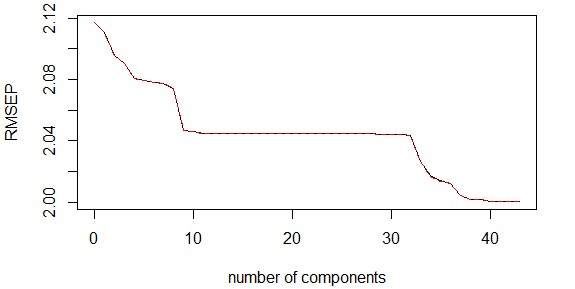
\includegraphics[scale=0.6]{pca_plot}
\label{fig:val}
\end{figure}



\subsection{Self Organising Map}
Due to the inability of PCR to identify a clear set of important variables, it was decided to construct a self-organising map (SOM) to assist in visualising any potential relationships between variables and yarn rating. The Kohonen package was used in R for this purpose \cite{WK2017}. Through trial and error, a grid size of 40X40, with a hexagonal topography was chosen to ensure instances were reasonably well distributed amongst nodes in the map. Separate heatplots for each individual variable were created from the output of the SOM algorithm. Each heatplot provided a visual representation of the distribution of its respective variable throughout the map. The positions of each instance from the dataset remained constant between heatmaps, which were coloured by the ‘density’ of the respective variables \cite{WK2017}. Correlations between variables can be qualitatively identified by studying the heatplots for similar or differing regions across two plots. No immediately obvious correlations were identified but some more subtle potential relationships are demonstrated in figure \ref{fig:SOM}.

\begin{figure}[h]
\caption{Heatplots for individual variables, as generated by a Self Organising Map}
\centering
\includegraphics[scale=0.45]{SOM_plots}
\label{fig:SOM}
\end{figure}

\vspace{5mm}

The inability to identify any clear correlations in the SOM heatplots further suggests that no single variable, or simple linear combination of independent variables has a significant influence on the yarn rating. As a result, more complex methods of analysis were necessary to identify possible non-linear relationships.

\section{Experiments}

All data acquisition, processing and analysis were performed using R. In order to reduce computation time, the data analysis was performed with virtual Linux machines using the Amazon EC2 cloud computing service. In all cases a single ‘4.8x Large’ instance (36 core Intel Xeon E5-2666 v3) \cite{Amazon2017} was used, running RStudio server. Prior to using EC2, attempts were made to train models on subsets of the data (with 10\% of the dataset used for training), however such models gave inconsistent results; therefore the entire dataset was used for model training and testing going forward. In order to effectively utilise the multi-core architecture, parallelisation of the code was necessary. In the case of the SVM and random forest models, parallelisation was carried out on the parameter grid search and the cross validation process. In order to implement this, the ‘doParallel’ library was used \cite{Calaway2017}. The deeplearning function in H2O, as used for the neural network, is implicitly parallel through the Hogwild! scheme \cite{Niu2011} so no further parallelisation of the code was required for NN models. Parallelisation came at the cost of reproducibility during parameter tuning since dynamic task allocation prevents subsequent runs of each program executing identically \cite{h2o2015}. However, parallelisation can be disabled and each of the best models may be re-created using the parameters found by each respective experiment.\\

Each method was limited to approximately 4 hours of computation time to allow a meaningful comparison between the methods. In all cases, some experimentation was carried out on a local machine with small subsets of the dataset to determine rough ranges for tuning parameters prior to training the full dataset on EC2.\\

5 fold cross validation was used throughout to evaluate each model. This was chosen as a compromise between evaluation quality and computation time. As is common for regression models, the Root Mean Squared Error (RMSE) was used as the evaluation metric for each model. Prior to computing any predictive models, the RMSE between all actual yarn ratings and the mean yarn rating was calculated, giving a RMSE of 0.675. As this was a trivial computation, this was used as a benchmark for model performance, with any RMSE below this considered an improvement.


\subsection{Support Vector Machine}
In order to implement a SVM, the e1071 library was used \cite{Meyer2017}. The cost and gamma parameters were tuned on the following grid:\\
\textbf{Cost:} 1 - 1e7\\
\textbf{Gamma:} 1e-5 - 1\\
The tuning range was so large because experiments on a subset of the overall dataset on a local machine failed to find a more localised search space over which the model performed well. Some parameter combinations would cause excessive runtime, therefore limiting the ability to search for an optimal range. This led to a total of 40 hours being necessary to execute the full experiment on EC2; however, on completion it was found that the best-performing individual model had required less than an hour to run, suggesting a better tuned search grid would require a similar running time to the subsequent methods.
  


\subsection{Random Forest}
By fitting numerous decision trees to the data and taking a consensus, Random Forests (RFs) often perform well with noisy data \cite{Follecco2008}. Previous studies have shown that extensive parameter tuning is often unnecessary to obtain good results \cite{Prior2006}. Indeed, the parameters which can be meaningfully tuned are limited to the ‘mtry’, ‘ nodesize’ and  ‘ntree’. These parameters represent the number of variables selected for each tree, the number of instances in the smallest node before terminating tree generation and the number of trees generated respectively \cite{Brieman2015}.
The randomForest package \cite{Brieman2015} was used to train Random Forest regression models on the dataset and tune the parameters. The mtry and nodesize parameters were tuned on the following grid:\\
\textbf{Mtry:} 10 - 40\\
\textbf{Nodesize:} 1 - 7\\
Experimentation with a subset of the data indicated that these parameter ranges gave the best results. It also indicated that tuning the 'ntree' parameter made little difference to overall performance, hence the use of the default value only in the final experiment. Models were trained and evaluated on the full dataset using EC2, which required approximately 3 hours of computation time.  

\subsection{Deep Neural Network}
To produce a predictive neural network, the ‘deepLearning’ function from the H2O package was used \cite{h2o2017,h2o2015}. This allowed the training of numerous networks with different parameter values. Due to the relatively large range of parameters available for tuning, a random search was carried out rather than a grid search. Parameters were randomly allocated for each candidate model from the following ranges:\\


\textbf{Number of hidden layers:} 1-4. \\
This was determined through experimentation on subsets of the overall dataset. Networks with more than 4 hidden layers performed poorly while requiring excessive computation time.\\

\textbf{Number of nodes per hidden layer:}
\begin{center}
\captionof{table}{search space for number of hidden nodes per layer}
\begin{tabular}{ | m{4em} | m{1cm}|m{1cm}|m{1cm}|m{1cm}|} 
\hline
\textbf{Hidden Layer} & 1 & 2 & 3 & 4 \\ 
\hline
\textbf{Number of Nodes}  & 10-100 & 10-100 & 10-80 & 5-30 \\ 
 \hline
\end{tabular}
\end{center}


\textbf{Activation function:} Rectifier, Rectifier With Dropout. \\
The rectifier type activation function is typical for regression models. The ‘rectifier with dropout’ activation function was also tried\cite{Kuo2016}\\

\textbf{Epochs:} 10. \\
Chosen as a compromise between computation speed and accuracy based on experimentation on subset of overall dataset.\\

\textbf{Input dropout ratio:} 0-0.1\\
This range provided reduced RMSE for given computation time during experimentation on subset of overall dataset.\\

\textbf{L1:} 1e-5 - 1e-2\\
This range provided reduced RMSE for given computation time during experimentation on subset of overall dataset.\\

\textbf{L2:} 1e-5 - 1e-2\\
This range provided reduced RMSE for given computation time during experimentation on subset of overall dataset.\\

\textbf{Distribution:} Gaussian\\
Other distributions were tried during the experimentation phase, however, the best performing models invariably used a Gaussian distribution.\\

\textbf{Adaptive learning rate:} TRUE. \\
This provided reduced RMSE for given computation time during experimentation on subset of overall dataset.\\

 Following experimentation on a small subset of the data to determine the above ranges for tuning parameters, the full training run was carried out on EC2. Computation time was limited to 4 hours, which resulted in the generation of 848 candidate models. This is significantly higher than the number of models generated by the SVM and Random Forest algorithms, however the benefit is offset by the larger parameter search space.




\section{Results}
The performance for the best model obtained by each method was as follows:
\begin{center}
\captionof{table}{Performance for each method}
\begin{tabular}{ | m{2cm} | m{1cm}| m{4.5cm}|} 
\hline
\textbf{Prediction method} & \textbf{RMSE} & \textbf{Parameters of best model}\\ 
 \hline\hline
Benchmark,  & 0.675 & \makecell{NA} \\ 
\hline
SVM & 0.582 &  \makecell{cost=100 \\  gamma=1e-5} \\ 
\hline
Random Forest & 0.551 & \makecell {mtry=10 \\ nodesize=7} \\ 
\hline
Deep Neural Network & 0.582 & \makecell{hidden layers=3 \\ hidden nodes=(98,40,43) \\  activation function = Rectifier \\ rate=0.005 \\  l1=2.2e-4 \\ l2=1.4e-3} \\
 \hline
\end{tabular}
\end{center}

\vspace{5mm}


The Random Forest model was the best predictor for yarn rating, giving a RMSE of 0.551. It is notable that the neural network and SVM gave similar results, whereas the Random Forest model performed significantly better. Plotting the predicted and actual ratings for a single test set (obtained from the cross validation fold allocations) gives an indication of the strengths of each model (figure \ref{fig:RP}.)

\begin{figure}[h]
\caption{Actual and predicted results for all instances from the testing set of one validation fold}
\centering
\includegraphics[scale=0.35]{results_plots}
\label{fig:RP}
\end{figure}

As each experiment involved the generation of multiple candidate models, the performance of the non-winning candidate models can be plotted to assess each algorithm’s sensitivity to parameter tuning.

\begin{figure}[h]
\caption{Performance of all models for full parameter search space}
\centering
\includegraphics[scale=0.6]{quantiles_plot}
\label{fig:QP}
\end{figure}

Within the parameter ranges tested, the SVM produced many models with extremely poor performance (RMSE greater than 1), suggesting a narrower parameter range should have been searched.  The Random Forest models outperformed the best SVM and Neural Network models even when sub-optimal parameters were used. This is illustrated in Figure \ref{fig:QP}. 



The e1071 implementation for SVMs does not include the ability to view variables by importance so only the NN and RF outputs may be compared for important variables.The plots in figure \ref{fig:VAR} show the relative variable importance for each method.

\begin{figure}[h]
\caption{Relative Variable Importances for NN and RF Methods}
\centering
\includegraphics[scale=0.6]{varimps_all}
\label{fig:VAR}
\end{figure}
\vspace{5mm}





\section{Discussion and Conclusions}
The yarn ratings on Ravelry are provided by a range of artists and hobbyists, all with different demands for a yarn. What one user considers a good yarn (for example low cost but low quality) may be considered poor by another. In addition, since many yarns are produced by other hobbyists, there is a tendency for ratings to be artificially high \cite{jforbes}. These factors made prediction of a yarn’s rating difficult and manifest as noise in the data.\\

\subsection{Model Performance}
The Random Forest method significantly outperformed a tuned Neural Network and SVM. Even without parameter tuning, a Random Forest would have outperformed the best performing models from the other two methods. Therefore, it can be said that for the given parameter search space and computational time, a Random Forest algorithm provides the best means to predict the rating for a given yarn. This does not necessarily mean it is the best of the three methods since a more extensive or optimised parameter search may allow either of the other two methods to exhibit an improvement in performance \cite{itsl} \\

Inspection of the plots in figure \ref{fig:RP} suggests that the SVM and RF models had the tendency to overfit on the ‘id’ attribute (for these plots, the instances were ordered by 'id' where the yarn ratings were equal - hence the tendency for predicted ratings to increase with instance number when yarn ratings are equal). The similarity in prediction pattern between the SVM and RF suggests a more optimised parameter search for the SVM method may have yielded better results. The NN models did not exhibit this behaviour, although this may simply be because the NN assigned the most importance to the 'grams' attribute which may have been overfitted to a similar degree. The NN method suffered from limited accuracy due to a tendency to constrain predictions to a relativley limited range, where both the SVM and particularly the RF method yielded less constrained predictions.

Although the Random Forest method gave the best accuracy, the reduction in RMSE over simply predicting the mean rating value for each yarn was only 0.124, from 0.675. As discussed, noise in the data will always impose a limit on the performance of predictive models for this dataset. As this is the first known study of this dataset, any significant improvement over guessing the mean was considered a success; however there is little doubt that other models could provide improved performance and the minimum practically achievable RMSE remains an open challenge.

\subsection{Variable Importance}
 Variable importance can only be compared between the NN and RF methods andis illustrated in figure \ref{fig:VAR}. In both cases, properties relating to the yarn product itself, rather than its actual composition accounted for the majority of the varience in ratings. For the RF model, three variables are immediately apparent as having high importance, these are the yarn id - which may be used as a proxy for time the yarn has been on the database; 'company yarn count' - which quantifies the number of other yarns the producing company already has on the database; and yardage - which is the overall length of yarn. None of these variables relate to a yarn's actual composition which indicates that Ravelry users are more likely to consider the nature of the producing company and the physical dimensions of the product, rather than the composition of the yarn itself. After these attributes, importance appears to fall off in a roughly linear manner. The most important variable which relates to yarn composition is the 'animal' variable (5th most important variable), which quantifies the amount of animal fibers in the yarn, this is followed by the 'acryllic' variable (6th most important variable). This suggests that although animal fibers are popular, cheap acryllic yarns also attract good ratings.  \\

Although the NN model gave poorer predictions on the yarn rating, it is interesting to note the variable importances used. Again, three variables are immediately apparent as being more important than others: 'grams', 'company yarns count' and 'Acryllic'. Subsequent importance dropoff is roughly linear, in keeping with the pattern observed from the RF. However, the NN model, assigned higher relative importance to the most important single variable than the RF model. Perhaps of more interest are the number of attributes relating to yarn fiber composition amongst the most important variables. Although product dimensions and company characteristics were of the most importance, the NN model assigned more importance to fiber composition than the RF model; with 'acryllic', 'merino', 'silk', 'animal' and 'cashmere' content all being in the top ten most important variables. With the exception of the 'acryllic' attribute, this suggests that after considering product dimensions and company characteristics, higher quality but more expensive yarns are generally favoured if the NN model is used for prediction. This difference also indicates that the NN model considered a fundementally different set of characteristics to be of importance to yarn rating, and therefore would merit further study in order to optimise this method for yarn rating prediction.





\section{Future Work}

While the models produced by this study were successful in identifying trends between yarn characteristics and user rating, any predictions made from these models are highly prone to error; and no single variable, or combination of variables, can be said to have an overriding influence on the rating. Indeed, the noisy nature of the yarn data implies a ceiling on the accuracy of any model, no matter how well trained it is.
However, the author acknowledges that improvements on the model accuracies presented here are certainly possible.  To obtain improved results while keeping computation time/cost constant, the following may be investigated in the future:

\subsection{Improved computational efficiency}
In all cases, models were trained and tested using parallel code running on 36 virtual CPU cores. The first step to improve efficiency would be to optimise the parallelisation. For example, for the SVM models, a single thread could delay the entire training run by occupying a single CPU core for several hours. If the SVM algorithm itself was parallelised, rather than just the parameter tuning and cross validation, a speedup could be achieved. In addition, it is recommended to use holdout validation rather than 5 fold cross validation during the parameter tuning stage since for future studies as this would allow 5 times as many parameters to be searched for the same computation time, albeit with reduced confidence in the model accuracies. Cross validation may then be used to validate the final model, therefore providing a higher confidence for accuracy.\\
An additional approach would be to use GPU processing \cite{zhou2013}. This would allow several thousand threads to be run simultaneously, therefore sampling from a much larger parameter grid and evaluation of a greater number of candidate models. GPU processing was not used for this study as libraries for GPU-optimised code are only available for limited applications in R currently. The deepLearning function in H2O may be run on a GPU through the deepwater package \cite{dh2o}, however this functionality was not used in order to allow for a fair comparison between models.
While it is certainly possible to manually create GPU-optimised functions in R, a better approach currently would be to use a dedicated package, such as TensorFlow or MXNet \cite{Abadi2015,Chen2015}.

\subsection{Parameter optimisation}
During generation of candidate neural network models, it was apparent that the method of randomly searching the parameter space was highly inefficient. Rather than a random or grid search (as used for the SVM and Random Forest models), some form of optimisation algorithm could potentially be used to select the best parameters. A genetic algorithm or simulated annealing are possible candidates and could be used in conjunction with GPU processing to ensure enough candidate models were generated to make the optimisation worthwhile \cite{Elyan2016,Coroiu2016}. This would allow for optimisation of parameters which were not tuned in this study.

\subsection{Alternative models}
This study focused on three distinct algorithms. Variations of these methods, or different methods entirely may give improved results. In the case of SVMs, different kernel methods may be used to the radial basis function applied here \cite{williams}. Numerous varieties of neural networks are available in addition to the deep backpropogation network used in this study, which have been shown to exhibit excellent performance for certain problem types\cite{nntypes}. Alternatives ensemble learning methods to the Random Forest model include Boosting, Bagging and Stacking\cite{williams,witten}. Other, completely different, machine-learning methods are available which may out-perform the Random Forest. Unsupervised clustering methods, for example, may give further insight into which variables are the most important for determining yarn rating \cite{witten}.

\subsection{Data processing}
The full dataset was not used for this study – approximately 52\% was omitted due to NA values. This decision was made as a trade off between computation time and model accuracy. Future studies may, however, benefit from assigning values to these NA entries in order to make use of the full dataset. This would require more comprehensive data processing since many of the rows containing NA values are invalid entries to the database.
Similarly, a number of text-based attributes were removed from the dataset. These contained information such as a written description of the yarn, and information on the supplying company. Consideration for these attributes could provide improved results but would require alternative methods of analysis.




% if have a single appendix:
%\appendix[Proof of the Zonklar Equations]
% or
%\appendix  % for no appendix heading
% do not use \section anymore after \appendix, only \section*
% is possibly needed

% use appendices with more than one appendix
% then use \section to start each appendix
% you must declare a \section before using any
% \subsection or using \label (\appendices by itself
% starts a section numbered zero.)
%



% Can use something like this to put references on a page
% by themselves when using endfloat and the captionsoff option.
\ifCLASSOPTIONcaptionsoff
  \newpage
\fi



% trigger a \newpage just before the given reference
% number - used to balance the columns on the last page
% adjust value as needed - may need to be readjusted if
% the document is modified later
%\IEEEtriggeratref{8}
% The "triggered" command can be changed if desired:
%\IEEEtriggercmd{\enlargethispage{-5in}}

% references section

% can use a bibliography generated by BibTeX as a .bbl file
% BibTeX documentation can be easily obtained at:
% http://www.ctan.org/tex-archive/biblio/bibtex/contrib/doc/
% The IEEEtran BibTeX style support page is at:
% http://www.michaelshell.org/tex/ieeetran/bibtex/
%\bibliographystyle{IEEEtran}
% argument is your BibTeX string definitions and bibliography database(s)
%\bibliography{IEEEabrv,../bib/paper}
%
% <OR> manually copy in the resultant .bbl file
% set second argument of \begin to the number of references
% (used to reserve space for the reference number labels box)
\begin{thebibliography}{30}

%\bibitem{IEEEhowto:kopka}
%H.~Kopka and P.~W. Daly, \emph{A Guide to \LaTeX}, 3rd~ed.\hskip 1em plus
%  0.5em minus 0.4em\relax Harlow, England: Addison-Wesley, 1999.
\bibitem{Hao2010}
L. Hao, Q. Guan-xiong, L. Xiao-jiu, C. Ling and W. Yuxiu, Quality grade recognition of knitted yarns by support vector machines, \emph{2010 International Conference on Computing, Control and Industrial Engineering},
 Wuhan,
 2010,
 pp. 49-51

\bibitem{Bo2010}
Z. Bo, Prediction of end breakage rates of cotton yarn in ring spinning processing by applying neural network approach and regression analysis theory, 
\emph{2012 International Conference on System Science and Engineering (ICSSE)},
 Dalian,
 Liaoning,
 2012, pp. 555-558.

\bibitem{chat2011}
R. Chattopadhyay, 4 - Artificial neural networks in yarn property modeling, In Woodhead Publishing Series in Textiles, edited by A. Majumdar, Woodhead Publishing, 2011, Pages 105-125, \emph{Soft Computing in Textile Engineering}, ISBN 9781845696634, http://dx.doi.org/10.1533/9780857090812.2.105.

\bibitem{basu2011}
A. Basu, 6 - Yarn engineering using an artificial neural network,
 In Woodhead Publishing Series in Textiles, Woodhead Publishing,
 2011, Pages 147-158,\emph{ Soft Computing in Textile Engineering},
 ISBN 9781845696634, http://dx.doi.org/10.1533/9780857090812.2.147.

\bibitem{forbes2014}
C. Forbes,
 Ravelry Application Developer and API License Agreement [online],
 Retrieved from \url{http://www.ravelry.com/wiki/pages/Legal%20:%20Application%20Developer%20and%20API%20License%20Agreement},
 (accessed 24/04/2017)

\bibitem{WK2017}
R.Wehrens, J.Kruisselbrink,
 2017,
 Package ‘Kohonen’ [online], Retrieved from \url{https://cran.r-project.org/web/packages/kohonen/kohonen.pdf} (accessed 17/04/2017)

\bibitem{Amazon2017}
Amazon, 
2017,
 Amazon EC2 Instance Types [online], 
Retrieved from \url{ https://aws.amazon.com/ec2/instance-types/}, 
(accessed 24/02/2017)

\bibitem{Calaway2017}
R. Calaway, S. Weston, D. Tenenbaum, Revolution Analytics, 2015, Package ‘doParallel’ [online], Retrieved from \url{ https://cran.r-project.org/web/packages/doParallel/doParallel.pdf}  (accessed 19/04/2017)

\bibitem{Niu2011} 
Benjamin Recht, Christopher Re, Stephen Wright, and
Feng Niu. Hogwild: A lock-free approach to parallelizing
stochastic gradient descent. In \emph{Advances in
Neural Information Processing Systems}, pages 693–701,
2011.

 \bibitem{Meyer2017}
D. Meyer, E. Dimitriadou, K. Hornik, A. Weingessel, F. Leisch, C. Chang, C. Lin,  2017, Package ‘e1071’ [online], Retrieved from \url{http://cran.rproject.org/web/packages/e1071/index.html}. (accessed 22.04.17).

\bibitem{Follecco2008}
A. Folleco, T. M. Khoshgoftaar, J. Van Hulse and L. Bullard, Software quality modeling: The impact of class noise on the random forest classifier, \emph{2008 IEEE Congress on Evolutionary Computation (IEEE World Congress on Computational Intelligence)}, Hong Kong, 2008, pp. 3853-3859.

\bibitem{Prior2006}
M. Prior and T. Windeatt, Parameter Tuning using the Out-of-Bootstrap Generalisation Error Estimate for Stochastic Discrimination and Random Forests, \emph{18th International Conference on Pattern Recognition (ICPR'06)}, Hong Kong, 2006, pp. 498-501.

 \bibitem{Brieman2015}
L. Brieman, L. Cutler, A. Liaw, M. Wiener, 2015, Package ‘randomForest’ [online], Retrieved from \url{ https://cran.r-project.org/web/packages/randomForest/randomForest.pdf}, (accessed 16/04/2017)

\bibitem{h2o2017}
The H2O.ai team, 2017, 'Package h2o' [online], Retrieved from \url{https://cran.r-project.org/web/packages/h2o/h2o.pdf},
(accessed 23/04/2017)

\bibitem{h2o2015}
A. Candel, J. Lanford, E. Ledell, V. Parmar, A.Arora, Deep Learning With h2o [online], Third Edition, H2O.ai.inc, Mountain View, USA,  Available at \url{https://h2o-release.s3.amazonaws.com/h2o/rel-slater/9/docs-website/h2o-docs/booklets/DeepLearning_Vignette.pdf}

\bibitem{Kuo2016}
C.-C. Jay Kuo, Understanding convolutional neural networks with a mathematical model, \emph{Journal of Visual Communication and Image Representation}, Volume 41, November 2016, Pages 406-413

\bibitem{zhou2013}
M. K. Zhou, F. Yin and C. L. Liu, GPU-Based Fast Training of Discriminative Learning Quadratic Discriminant Function for Handwritten Chinese Character Recognition, \emph{2013 12th International Conference on Document Analysis and Recognition}, Washington, DC, 2013, pp. 842-846.

 \bibitem{Abadi2015}
Abadi et al, 2015, TensorFlow: Large-Scale Machine Learning on Heterogeneous Distributed Systems, 
arXiv:1603.04467  

\bibitem{Chen2015}
Tianqi Chen, Mu Li, Yutian Li, Min Lin, Naiyan Wang, Minjie Wang, Tianjun Xiao, Bing Xu,
Chiyuan Zhang, and Zheng Zhang. Mxnet: A flexible and efficient machine learning library for
heterogeneous distributed systems. arXiv:1512.01274, 2015a.

\bibitem{Elyan2016}
E. Elyan. and M.M.Gaber, 2017. A genetic algorithm approach to optimising random forests applied to class engineered data. \emph{Information sciences} [online], 384, pages 220-234. Available from: https://dx.doi.org/10.1016/j.ins.2016.08.007

\bibitem{Coroiu2016}
A. M. Coroiu, Tuning model parameters through a Genetic Algorithm approach, \emph{2016 IEEE 12th International Conference on Intelligent Computer Communication and Processing (ICCP)}, Cluj-Napoca, 2016, pp. 135-140.

\bibitem{itsl} 
G. James, D. Witten, T. Hastie, R. Tibshirani, 2013, \emph{An Introduction to Statistical Learning}, New York, Springer.

 \bibitem{dh2o}
A. Candel, Deep Learning in H2O using Native GPU Backends, 2017, Github repository, available at \url{https://github.com/h2oai/deepwater}

\bibitem{williams}
G. Williams, 2011, \emph{Data Mining With Rattle and R}, New York, Springer

\bibitem{witten}
A. Witten, E. Frank, M. Hall, 2011, \emph{Data Mining: Practical Machine Learning Tools and Techniques}, Third Edition, Burlington, Elsevier

\bibitem{nntypes}
L. Deng, G. Hinton and B. Kingsbury,
 New types of deep neural network learning for speech recognition and related applications: an overview, \emph{2013 IEEE International Conference on Acoustics, Speech and Signal Processing}, Vancouver, BC, 2013, pp. 8599-8603.

\bibitem{jforbes}
J. Forbes, 2016, Ravelry’s Wiki : A Community Edited Guide [online], Retrieved from \url{http://www.ravelry.com/wiki/pages/HomePage} (accessed 15/04/2017)

\end{thebibliography}

% biography section
% 
% If you have an EPS/PDF photo (graphicx package needed) extra braces are
% needed around the contents of the optional argument to biography to prevent
% the LaTeX parser from getting confused when it sees the complicated
% \includegraphics command within an optional argument. (You could create
% your own custom macro containing the \includegraphics command to make things
% simpler here.)
%\begin{IEEEbiography}[{\includegraphics[width=1in,height=1.25in,clip,keepaspectratio]{mshell}}]{Michael Shell}
% or if you just want to reserve a space for a photo:



% You can push biographies down or up by placing
% a \vfill before or after them. The appropriate
% use of \vfill depends on what kind of text is
% on the last page and whether or not the columns
% are being equalized.

%\vfill

% Can be used to pull up biographies so that the bottom of the last one
% is flush with the other column.
%\enlargethispage{-5in}



% that's all folks
\end{document}